\documentclass[
    11pt,
    a4paper,
    sfdefaults=false,
    toc=chapterentrywithdots,
    twoside,openright,
    titlepage,
    parskip=half,
    headings=normal,  % reduces heading size
    listof=totoc,
    bibliography=totoc,
    index=totoc,
    captions=tableheading,  % caption below table
    chapterprefix,
    listof=flat,
    final
]{scrbook}


% details about your thesis
\newcommand{\titel}{RaspberryPi CyberSec Lab: Development of a Penetration Testing Platform}
\newcommand{\artderarbeit}{Bachelorarbeit}  % {Bachelorarbeit,Masterarbeit}
\newcommand{\autor}{Jonas Schmitt}
\newcommand{\studiengang}{Elektro- und Informationstechnik}  %{Informatik,Wirtschaftsinformatik,Medieninformatik}
\newcommand{\matrikelnr}{3619551}
\newcommand{\erstgutachter}{Prof. Dr. Aykan D. Inan}
\newcommand{\zweitgutachter}{Jörg Arndt}
\newcommand{\logo}{figures/TH-Nuernberg-RGB.png}
\newcommand{\keywords}{AI, Quantum Computing, Data Driven Businesses, Deep Learning, Self Improvement, Diversity} 

% custom head and foot
\usepackage[automark]{scrlayer-scrpage}
\pagestyle{scrheadings}
\ohead{\headmark}
\chead{}
%\ohead{\pagemark}
\renewcommand*\chaptermarkformat{\chapappifchapterprefix{\ }% 
  \thechapter.\enskip}

\RedeclareSectionCommand[tocindent=15pt]{section}
\RedeclareSectionCommand[tocindent=40pt]{subsection}
%\RedeclareSectionCommand[tocnumwidth=70pt]{chapter}

\usepackage{scrhack}

% other packages
\usepackage[utf8]{inputenc}
\usepackage[T1]{fontenc}
\usepackage{lmodern,relsize,textcomp,csquotes}
\usepackage{amsmath,amsfonts}
\usepackage[english]{babel}  % flip for German thesis
\usepackage[final]{graphicx}
\usepackage{setspace,geometry,xcolor}
\usepackage{makeidx}
\usepackage{paralist,ifthen,todonotes}
\usepackage{url}
\usepackage[toc]{glossaries}
\usepackage{pdfpages}
\usepackage{multicol}
\usepackage{microtype}

% table setup
\usepackage{longtable}
\usepackage{array}
\usepackage{ragged2e}
\usepackage{lscape}
\usepackage{booktabs}
\newcommand{\ra}[1]{\renewcommand{\arraystretch}{#1}}

% pdf hyperref
\usepackage[
    bookmarks=true,
    bookmarksopen=true,
    bookmarksnumbered=true,
    bookmarksopenlevel=1,
    pdftitle={\titel},
    pdfauthor={\autor},
    pdfcreator={\autor},
    pdfsubject={\titel},
    pdfkeywords={\keywords},
    pdfpagelabels=true,
    colorlinks=true,
    linkcolor=red,
    urlcolor=magenta,
    anchorcolor=black,
    citecolor=cyan,
    filecolor=magenta,
    menucolor=red,
    plainpages=false,
    hypertexnames=true,
    linktocpage=true,
]{hyperref}

\usepackage{cleveref}

% configure your listings style

\usepackage{inconsolata}
\usepackage{xcolor}
\usepackage{listings}
\lstset{
	tabsize=3,
	extendedchars=true,
	frame=single,
	showstringspaces=false,
  breaklines=true,
	numbers=left,
	breakautoindent=trubreaklines=true,                     % Enable line breakinge
  basicstyle=\ttfamily\fontsize{8.5}{9}\selectfont,
  keywordstyle=\color{cyan!75!black}\bfseries,
  commentstyle=\color{green!75!black},
  stringstyle=\color{orange},
  numberstyle=\tiny\color{gray}
}

% page setup
% \setlength{\topskip}{\ht\strutbox}
\geometry{paper=a4paper,left=2.5cm,top=3.0cm,bindingoffset=.8cm}
\onehalfspacing
\frenchspacing
\clubpenalty = 10000
\widowpenalty = 10000 
\displaywidowpenalty = 10000

% some commands
\newcommand{\ua}{\mbox{u.\,a.\ }}
\newcommand{\zB}{\mbox{z.\,B.\ }}
\newcommand{\dahe}{\mbox{d.\,h.,\ }}
\newcommand{\bzw}{\mbox{bzw.\ }}
\newcommand{\bzgl}{\mbox{bzgl.\ }}
\newcommand{\eg}{\mbox{e.\,g.\ }}
\newcommand{\ie}{\mbox{i.\,e.\ }}
\newcommand{\wrt}{\mbox{w.\,r.\,t.\ }}
\newcommand{\etal}{\mbox{\emph{et\,al.\ }}}


% load glossary entries
\makenoidxglossaries
\loadglsentries{glossary}

\begin{document}

\setcounter{secnumdepth}{3}  % numerate subsections
\setcounter{tocdepth}{2}  % ...but don't include them in toc

\frontmatter
\include{cover}\cleardoublepage

% download the following form (requires VPN) and complete it (hit save in your editor)
% https://intern.ohmportal.de/fileadmin/Public_Docs/SB/SB_0009_FO_Pruefungsrechtliche_Erklaerung_und_Erklaerung_zur_Veroeffentlichung_der_Abschlussarbeit_public.pdf
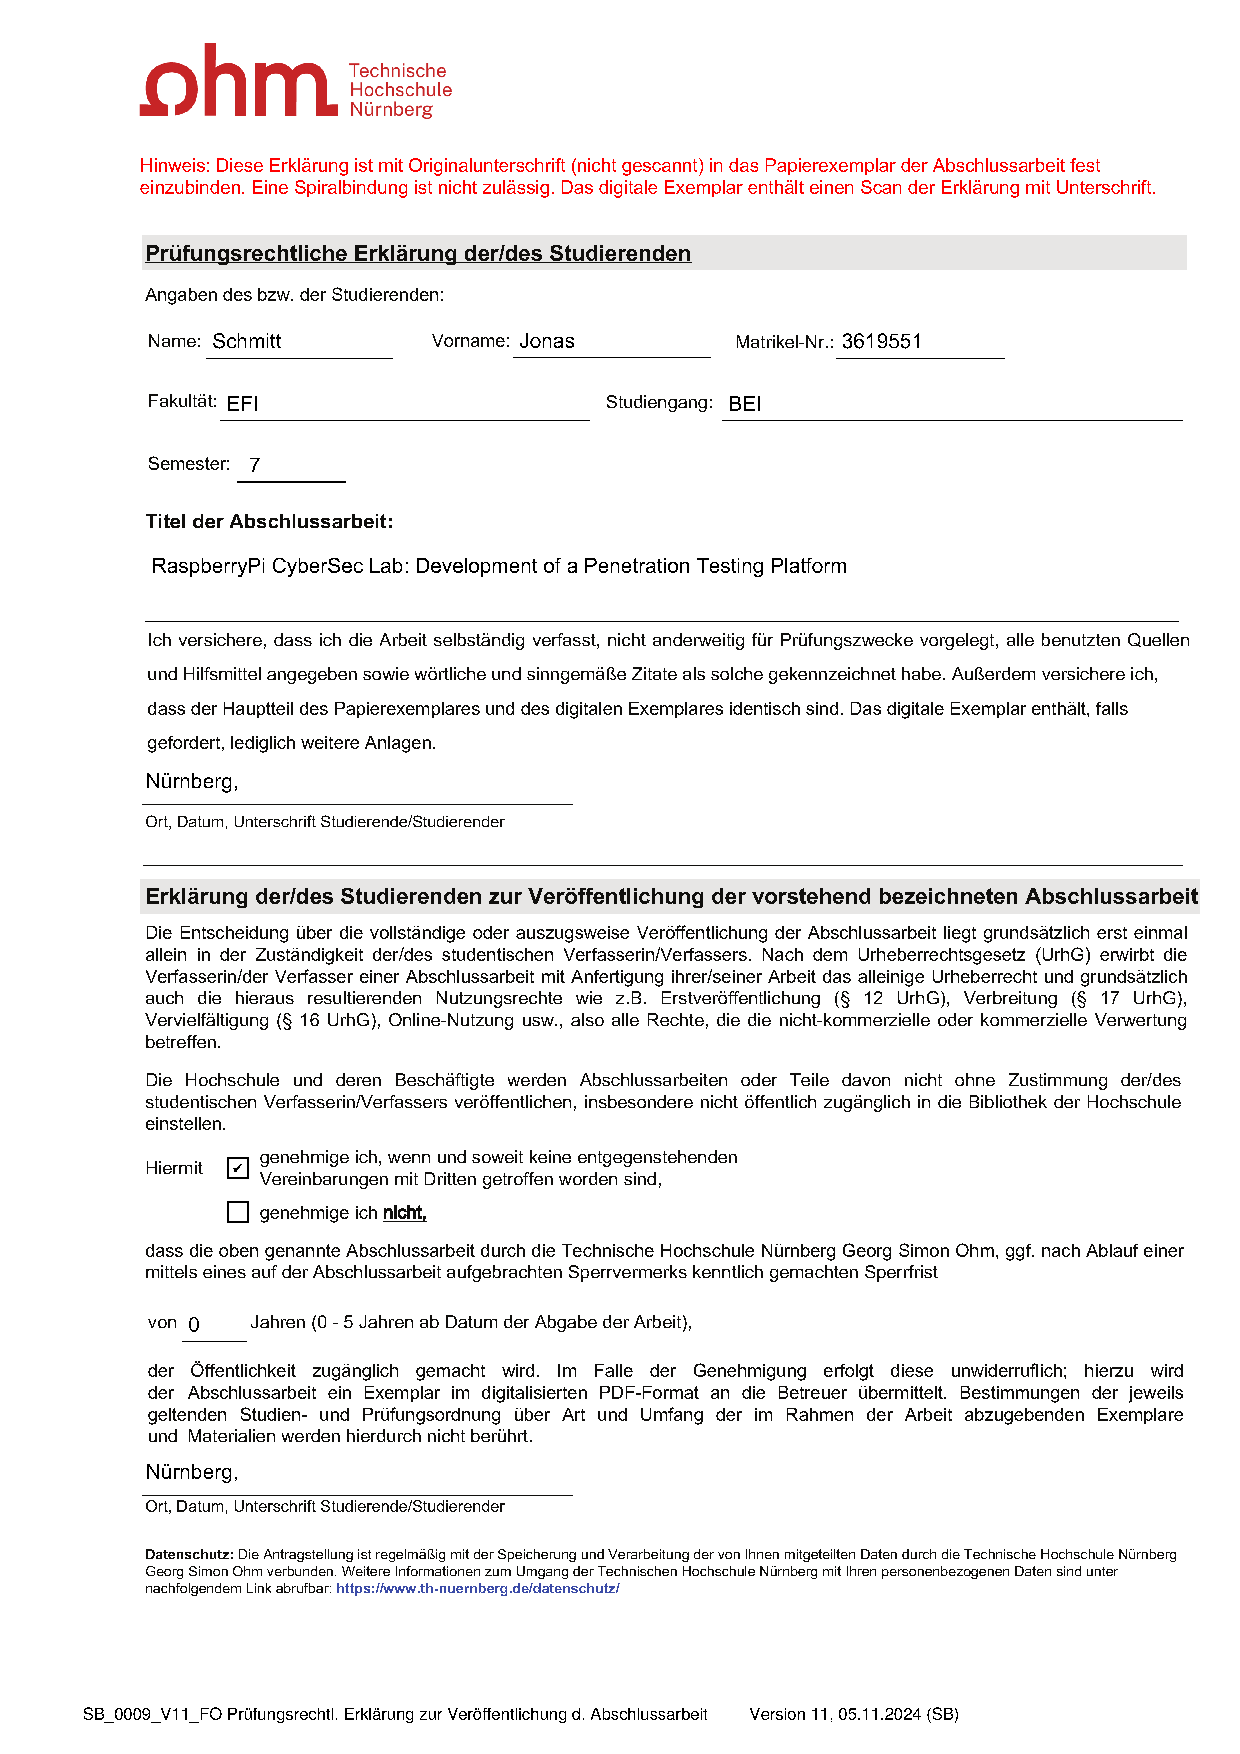
\includepdf{SB_0050_FO_Pruefungsrechtliche_Erklaerung_und_Erklaerung_zur_Veroeffentlichung_der_Abschlussarbeit_Jonas_Schmitt.pdf}\cleardoublepage

\thispagestyle{empty}

\section*{Abstract}\label{sec:abstract}
This thesis documents the development and testing of the RaspberryPI Cyber Security Laboratory (RCSL).
The RCSL is imagined as a testing platform for demonstration and practice purposes of Cybersecurity in various IT applications.

An expandible software architecture is developed, which focuses on usability and includes features for the creation of test environments in the WiFi and web application domain.
Development and functionality are documented, highlighting the challenges encountered along the process.

Testing is conducted in the form of cracking the WEP and WPA/WPA2 network standards and the results are evaluated.
Along testing several faults in the system were discovered and mostly corrected.
The results show the RCSL to be capable of establishing testing environments for WiFi security.

Proposed usecases for the RCSL include demonstration and hands-on practice in cybersecurity and software development education.
Future improvement and expansion of the project are recommended.


\newpage

\section*{Kurzdarstellung}
\label{sec:kurzdarstellung}
Diese Arbeit dokumentiert die Entwicklung und Erprobung des RaspberryPI Cyber Security Laboratory (RCSL).
Das RCSL ist als Testplattform für Demonstrations- und Übungszwecke von Cybersecurity in verschiedenen IT-Anwendungen gedacht.

Es wird eine erweiterbare Software-Architektur entwickelt, die sich auf die Benutzerfreundlichkeit konzentriert und Funktionen für die Erstellung von Testumgebungen im WiFi- und Web-Anwendungsbereich enthält.
Entwicklung und Funktionalität werden dokumentiert und die dabei aufgetretenen Herausforderungen aufgezeigt.

Als Tests werden das cracking der Netzwerkstandards WEP und WPA/WPA2 durchgeführt und die Ergebnisse ausgewertet.
Während der Tests wurden mehrere Fehler im System entdeckt und größtenteils behoben.
Die Ergebnisse zeigen, dass das RCSL in der Lage ist, Testumgebungen für WiFi-Sicherheit einzurichten.

Vorgeschlagene Anwendungsfälle für den RCSL sind Demonstrationen und praktische Übungen in der Cybersecurity- und Softwareentwicklungslehre.
Zukünftige Verbesserungen und Erweiterungen des Projekts werden empfohlen.\cleardoublepage

\tableofcontents

\mainmatter
\include{content/1_intro}
\chapter{Basics of Cybersecurity}\label{ch:basics_cybersec}
This chapter briefly explains the terms of IT- and Cybersecurity and gives an overview of their goals and methods.
A summary of common threads in the Cybserspace is given as well.

\section{IT Security}
IT Security describes the protection of digital data and computer- and communication systems from unauthorized access.
Different principles are adhered to and methods and techniques applied in order to prevent the theft, interception, manipulation and loss of data and systems. \cite{IT_Basiswissen}

\section{Cybersecurity}
IT- and Cybersecurity are similar in that both have the same goals and apply the same principles and methods.
While IT Security focuses on classical computer systems and networks, Cybersecurity focuses on data and systems in the Cyberspace.
Included in the Cyberspace are all systems and data connected to the internet.

\subsection{Goals}
The goals of Cybersecurity include but are not limited to the well known CIA triad, which is an acronym for Confidentiality, Integrity, and Availability \cite{Oriyano_2017}.
Confidentiality describes data only beeing accessible by the persons, who are meant to do so.
Integrity describes data beeing unchanged after storage or transmission, meaning the data was not corrupted or manipulated.
Availability describes data and systems beeing accessible with the expected performance, whenever required. 

\subsection{Methods}\label{ssec:cs_methods}
Some methods for achieving the goals of Cybersecurity are:

\begin{itemize}
    \item Security Awareness is the knowledge of the threads present in the Cyberspace and methods for protection.
    "Awareness of the risks and available safeguards is the first line of defence for the security of information systems and networks" \cite[page~26]{IT_Basiswissen}.
    \item Encryption is a cryptographic\footnote{cryptography = science of secretive writing} method, which takes the readable data, called plaintext, and makes it unreadable for anyone besides the legitimate recipient.
    The encrypted text is called ciphertext and can be made readable again, by decrypting it.
    To en- and decrypt a message, the sender and recipient have knowledge of a secret, often a passphrase, which controls en-/decryption and is called key. \cite[page~1]{Watjen_2018}
    \item Authentication is the act of a user "performing some sort of action which proves that the claim a user is making about who they are is actually valid" \cite{Oriyano_2017}. 
    This is oftentimes done through the use of a password, in the case of WiFi networks, the knowledge of the password proves, that a user is allowed to access the network.
    \item Pentesting is a method to audit the security of a system or network. 
    It involves a security professional performing various types of attacks to discover weaknesses in soft- and hardware.
    \item Monitoring with anomaly detection can be used to detect the unauthorized access of systems and networks.
    In the network domain so called Intrusion Detection Systems (IDS) employ predictive models to recognize malicious activity inside a network \cite{geeksforgeeks_ids}.
    \item Incident Response is performed in case of a system breach in order to limit damage and secure the system.
\end{itemize}

\section{Threads and Risks in the Cyberspace}
There are various types of Cybercriminals with different motives and intentions.
Motives of Cybercriminals can vary but commonly are financial, political, social or military.
With these motives the intentions of an attack often are:
\begin{multicols}{2}
    \begin{itemize}
        \item blackmail
        \item espionage
        \item theft
        \item fraud
        \item sabotage
        \item corruption and insider deals
    \end{itemize}
\end{multicols}

The successrate and risk of an attack are in large parts determined by a targets attack area, which is the combination of the present vulnerabilities and attack vectors.
The term vulnerability describes a weakspot, which can be exploited by the attacker to break or circumvent security mechanisms.
An attack vector is the approach, an attacker takes for carrying out an attack.
With regards to Network Security some common attack vectors are:

\begin{itemize}
    \item Denial of Service (DoS) attacks availability by preventing or limiting the functional capability of a system.
    \item Cracking describes the act of breaking or circumventing security mechanisms, e.g. reverse engineering passwords.
    \item Brute-Force is a technique for reverse engineering passwords by trail-and-error.
    \item Spoofing refers to fakeing identities, achieved by the obfuscation of the own identity or the replication of another identity.
    \item Sniffing is the action of collecting all openly available data, e.g. recording unecrypted wifi frames.
    \item Man-in-the-Middle (MitM) attacks involve injection of a malicious device into a line of communication, which subsequently can manipulate and eavesdrop on the traffic.
    \item Social Engineering is a form of manipulation which abuses psychological mechanisms like trust, curiosity or shock to exploit victims.
\end{itemize}

\cite[page~16-20]{IT_Basiswissen}



\chapter{Basics of Wi-Fi}\label{ch:basics_wifi}

This chapter explains the basics of Wi-Fi technology.
Insight into the history and development of Wi-Fi is given and its functionality and security mechanisms are briefly explained.

\section{History}

In 1985 the American Federal Communications Commission ruled several bands in the 2.4 GHz radio band to be unlicensed, meaning everyone can broadcast radio signals in these frequencies.
At the beginning of the 90s, this led to the development of different wireless communication protocols by multiple companies.
To ensure interoperability between these protocols, the IEEE 802.11 standard was created and released, and WLAN was born.
In 1999 the Wi-Fi Alliance (WFA) was founded to further improve compatibility, nowadays consisting of over 750 international companies. \cite[page~1-3]{Sankaran_Gulasekaran_2021}, \cite{Wikipedia_2025}

Since its inception over 25 years ago, Wi-Fi has gone through constant development, leading to six major generations of the technology.
Improvements in speed, efficiency, and security have led to the technology becoming a "fundamental utility [...], that everyone [...] expects to be available everywhere" \cite[page~1]{Sankaran_Gulasekaran_2021}.
Wi-Fi connects billions of devices, like computers, smartphones, game consoles, or IoT devices to the internet, generating a value of around 4.9 trillion USD worldwide \cite[page~1]{Sankaran_Gulasekaran_2021}.

Wi-Fi operates at the physical (PHY) and the medium access control (MAC) layer of the OSI model, sending Ethernet frames over radio waves in the 2.4 and 5 GHz frequency band. 
The MAC layer is responsible for setting rules on transmission and reception of data, connection management and power management.
Data sent on the MAC layer then gets converted to radio waveforms by the PHY layer, which is also responsible for converting received data back to the MAC protocol. \cite[page~4-7]{Sankaran_Gulasekaran_2021}

\section{MAC layer}
Devices in the MAC layer are addressed with a MAC address, which consists of 12 hexadecimal characters and is unique for every network interface controller (NIC).

A MAC address could look like this: \lstinline[basicstyle=\ttfamily\small]|61:A3:E2:73:9A:F3|.

\subsection{Architecture}

Commonly, Wi-Fi networks have access points (AP), which are connected to the internet via ethernet, and stations (STA), which are provided with internet access over Wi-Fi by the AP.
Wi-Fi has a MAC layer, which is designed to be flexible and can be configured in the following topologies:
\begin{itemize}
    \item \textbf{BSS}: Basic Service Set
    \item \textbf{IBSS}: ad hoc / peer-to-peer / Independent BSS
    \item \textbf{WDS}: Wireless Distribution System
    \item \textbf{MBSS}: Mesh BSS
\end{itemize}


BSS describes the most common and basic configuration, where multiple STAs are connected to one AP, which has wired connection to the internet.
IBSS networks don't have any APs, instead the STAs are connected directly to each other.
WDS can be used when the reach of an AP needs to be extended, but there is no wired connection available. 
A secondary AP can be installed, which receives backhaul connection from the first AP.
Mesh Networks are complex BSS networks with multiple APs, which the STAs can hop between.
This type of network can improve the signal coverage and resilience and is often used in companies or public institutions. \cite[page~8-9]{Sankaran_Gulasekaran_2021}

\subsection{MAC Frames}

\begin{figure}[h]
    \centering 
    
\includegraphics[width=\linewidth]{figures/Abbildungen/MAC_Frame.pdf}
    \caption{MAC Frame of BSS Wi-Fi Network}
    \label{fig:mac_frame}
\end{figure}

When data is sent over the MAC layer, it gets divided into chunks, which are called MAC Frames.
MAC Frames have three components: the header, the body, and the frame check sequence.
The header contains information about the source and destination, the sequence and several control functions.
In a BSS network it has the following functions:

\begin{itemize}
    \item \textbf{Frame Control} contains 16 Bits which serve different control functions
        \subitem \textbf{Protocol Version} describes which version of the MAC protocol this frame uses
        \subitem \textbf{Type} describes the type of MAC frame is being used: there are data, management, control and acknowledgment frames
        \subitem \textbf{Subtype} describes the subtype of the frame, e.g. association request or beacon frame
        \subitem \textbf{From/to ds} indicates the direction of travel
        \subitem \textbf{More Fragment} indicates more following fragments
        \subitem \textbf{Retry} indicates that the current frame is a retransmission
        \subitem \textbf{Power Management} gives information about the power state of the STA
        \subitem \textbf{More Data} indicates more frames are to be transmitted 
        \subitem \textbf{Protected Frame} indicates whether a frame is encrypted
        \subitem \textbf{Order} set to 1 if the order of processing is important
    \item \textbf{Duration} indicates the time of the transmission, therefore how long the medium is occupied
    \item \textbf{Address 1} contains the receiver address (RA), which can be the MAC address of the destination STA or the BSSID of the AP, depending on the direction, the frame travels
    \item \textbf{Address 2} contains the transmitter address (TA), which can be the BSSID or the source address.
    \item \textbf{Address 3} contains either the source or destination address
    \item \textbf{Sequence Control}
        \subitem \textbf{Fragment Number} ensures the correct processing sequence of the fragments
        \subitem \textbf{Sequence Number} number of the frame
\end{itemize} 

The frame body then contains the payload, meaning the actual information to be sent.
Every type of MAC frame is configured a different way to suit their specific function.
"While data frames are meant to carry data, management frames are used for connection management and control frames [...] for triggering specific actions.
Control frames have a smaller MAC header and no payload data [...].
Management frames have a structured payload composed of some fixed length fields and one or more variable length fields called information elements (IEs)" \cite[page~12]{Sankaran_Gulasekaran_2021}

After the frame body comes the frame control sequence (FCS), which ensures the integrity of the frame.
The FCS is a cyclic redundancy check (CRC), which is a number calculated from the frame header and body content.
When the frame is compromised in traffic, the result of the CRC changes, therefore the faulty frame can be identified. \cite{GeeksforGeeks_2023} \cite[page~10-12]{Sankaran_Gulasekaran_2021}

\subsection{Medium Access}
In LAN and WLAN networks, all devices share the same medium, therefore only one device at a time can transmit information.
Ethernet networks use full-duplex transceivers, meaning a device can transmit and receive data at the same time.
This allows the transceiver to transmit and simultaneously listen for collisions with other frames.
Collision detection is quite effective, but can not be used in Wi-Fi networks because Wi-Fi transceivers are only capable of half-duplex transmission.
Wi-Fi instead uses a medium access control referred to as carrier sense multiple access collision avoidance (CSMA-CA).

When using this technique, the medium gets blocked during transmission and is freed by an acknowledgment frame, sent by the receiving device.
All STAs start off in the random backoff state, where they listen for traffic.
After the random backoff counter has expired and no traffic is present, the STA will start transmission.
CSMA-CA can be described by the way "humans converse in a group, where every individual would first listen to check if someone else is talking, wait for the person talking to finish, and then start talking after a brief random pause" \cite[page~12]{Sankaran_Gulasekaran_2021}. \cite{Oriyano_2017} \cite[page~12-17]{Sankaran_Gulasekaran_2021}

For addressing a STA, its MAC address needs to be known.
For sharing the MAC address of a STA with all other STAs on the network, the Address Resolution Protocol (ARP) is employed, which broadcasts the STAs MAC addresses, allowing all other devices to save it.

\subsection{Connection Establishment and Termination}
Before a connection can be established, the STA first needs to discover the AP it wants to connect to.
This can be done by either active or passive scanning of all available channels.

During active scanning, the STA transmits a management frame, called probe requests on all channels to all SSIDs in the vicinity.
The APs answer with a probe response frame, which contains the AP's SSID, BSSID and its capabilities.

Passive scanning works by the STA listening for beacon frames.
Beacon frames are periodically sent out by APs and also contain information on SSID, BSSID and capability. \cite[page~18]{Sankaran_Gulasekaran_2021}

Once the desired network is discovered, the STA decides which AP to connect to, based on parameters, like the receive signal strength indicator (RSSI) or the APs capacity, performance and security.
The STA then sends an authentication request, which the AP gives an authentication response to.
If the credentials of the STA are valid and the authentication is successful, the STA proceeds to send an association request.
The association response, sent by the AP, then indicates if the connection was established successfully.

To terminate a connection, either the STA or the AP can send a disassociation or deauthentication frame, "containing a reason code that specifies the reason for termination" \cite[page~20]{Sankaran_Gulasekaran_2021}. \cite[page~19]{Sankaran_Gulasekaran_2021}

\begin{figure}[h]
    \centering 
    
\includegraphics[width=0.6\textwidth]{figures/Abbildungen/Wifi_Establishment.pdf}
    \caption{Connection Establishment}
    \label{fig:connection_establishment}
\end{figure}

\section{PHY layer}
The Wi-Fi PHY layer is based on radio frequency (RF), therefore Wi-Fi transceivers contain a transmitter and receiver circuit, as well as an antenna.
When sending data, MAC frames are encoded and modulated onto an RF waveform, which is then transmitted via the antenna.
On arrival of data, the receiver circuit decodes the data, extracts the MAC frame, and provides it to the MAC layer.
The first generations of Wi-Fi used to transmit in the 2.4 GHz band, but due to it being used by many other devices, such as cordless phones, computer peripherals, Bluetooth devices or microwave ovens, Wi-Fi 4 started using the 5 GHz band, in order to improve connectivity. \cite[page~5,34,35]{Sankaran_Gulasekaran_2021}
With every generation of Wi-Fi, the PHY layer components are modified to improve performance and efficiency, but due to the PHY layer not being majorly significant for cybersecurity, it will not be described further in this thesis.

\section{Security}

Through the widespread adoption of Wi-Fi technology, for example in smart homes, infrastructure, public spaces, industry, and governments, the security of Wi-Fi networks plays an ever increasing role.
Therefore, principles of cybersecurity need to be applied in order to guarantee that networks are safe, reliable, and performant.
Because of its wireless nature, "[i]t is difficult to confine the data-carrying radio waves to be within the physical security perimeter of [an] organizsation" \cite[page~103]{Sankaran_Gulasekaran_2021}, so anyone in the vicinity of a Wi-Fi network could just intercept and manipulate network traffic.
To ensure integrity and confidentiality, Wi-Fi two main security mechanisms, which are encryption and authentication. \cite[page~103]{Sankaran_Gulasekaran_2021}

\textit{Note: Since this thesis is focused on private networks, the following summary of Wi-Fi security mechanisms will not include enterprise authentication protocols.}
    
\subsection{Encryption}

The first "secure" Wi-Fi standard, called Wired Equivalent Privacy (WEP) uses a shared key, with a RC4 stream cipher algorithm for message encryption and a 32-Bit CRC as a integrity check (IC).
Due to several vulnerabilities of WEP, including the RC4 algorithm, a lack of authentication and no key management, the second standard, wireless protected access (WPA), was developed.

WPA still uses the RC4 cipher for compatibility reasons, but the encryption mechanism was updated, now called Temporal Key Integrity Protocol (TKIP), it uses a pairwise master key, which is generated for each STA after it has authenticated successfully.
TKIP also dynamically changes the encryption key for each packet, which in combination with a longer 128-Bit pre-shared key (PSK) fixed some of the weaknesses of WEP. \cite{Oriyano_2017}

WPA2 could be considered as the first proper Wi-Fi security standard since it replaced the weak RC4 algorithm with AES-CCMP\footnote{Advanced Encryption Security - Counter mode CBC MAC Protocol} encryption.
AES-CCMP encrypts data blockwise and uses a combination of substitution and transposition algorithms to achieve high security.
WPA2 security also added protected management frames, so not only data frames, but also management frames are encrypted.
This helps to secure networks against DoS attacks with deassociation or deauthentication frames.

The newest Wi-Fi security standard is WPA3, which aims to fix vulnerabilities of WPA2 and future-proof the technology.
Most changes for WPA3 have been made in authentication mechanisms, WPA3 added the optional support of AES-GCMP\footnote{AES - Galois Counter Mode Protocol} encryption, which is more performant and even safer than AES-CCMP. \cite[page~103-117]{Sankaran_Gulasekaran_2021}


\subsection{Authentication}

WEP authentication is only one-sided, where STA has to encrypt a package with the correct key, in order to complete association with the AP. 
The same key is used for encryption, making the whole system vulnerable when either the authentication or the encryption is exploited. 

WPA and WPA2 networks use an authentication mechanism that is two-sided, where STA and AP exchange identity and capability.
After entering the correct passphrase a password-based key derivation function then generates the PSK for encryption. 
This works by deriving the PSK "as a function of the Wi-Fi password, SSID, and SSID length using a password-based key derivation function" \cite[page~106]{Sankaran_Gulasekaran_2021}.

Because the PSK is transmitted during the handshake on connection establishment, PSK is potentially vulnerable to offline and dictionary attacks when a weak passphrase is used.
To future-proof the technology, WPA3 replaces PSK with Simultaneous Authentication of Equals (SAE).
SAE works by choosing an element from a finite cyclic group (e.g., a point on an elliptic curve) based on the password and performing a Diffie-Hellman exchange to generate a pairwise master key.
This mechanism allows authentication without the transmission of any information related to the password and is performed for every session to ensure forward security.
\cite{Oriyano_2017}, \cite[page~115-116]{Sankaran_Gulasekaran_2021}, \cite{SAE}

\textit{Note: A full summary of the different security specifications of each Wi-Fi generation, can be found in \cref{tab:wifi_security}.}

\include{content/4_documentation}
\include{content/5_development}
\chapter{Pentesting}\label{ch:testing}
This chapter describes the pentesting of the WiFi enviroments, established with the RCSL.
It starts of by explaining some common (WiFi-) network attacks, of which the cracking of WEP and WPA/WPA2 are then tested on the RCSL and the results documented.

\section{Attacks}
WiFi attacks can take many different forms, depending on the type of attack and and which mechanism it tries to break.
There are attacks aimed at breaking the Access Controls, Integrity Controls, Confidentiality or Availability. \cite{Oriyano_2017}
The following selection of attacks quite nicely depicts the different vectors an attacker can take to hack a WiFi network and its STAs.

\subsection{War Driving}
War Driving describes the act of gathering information on WiFi networks in larger numbers in order to locate specific or weak targets.
This is done by traversing areas of interest with data collection equipment, which collects information about every network coming into range.
After capturing and mapping as many WiFi networks as possible, a more sophisticated attack can be launched on the captured networks or the data can be sold on the black market. \cite{Oriyano_2017}

\subsection{Rogue Access Point and Evil Twin}
When using Rogue Access Points, attackers place extra APs onto a network, trying to stay undetected and get STAs to connect to the malicious AP.
This can for example be done by connecting an AP to an open and unprotected LAN port inside a public or company building.
Once a STA has connected to the rogue AP it acts as a MITM, allowing the attacker to manipulate or eavesdrop on the traffic.

Evil Twins have some similarity to Rogue Access Points, in that they also pretend to be a legitimate part of an existing network.
Different to Rogue APs, Evil Twins do not connect to the legitimate network, but instead spoof wireless networks, providing a stronger signal, to again get STAs to connect to it.
Some attackers might also use a deauthentication flood to get STA disconnected from their genuine AP and autoconnect to the malicious one.

Because they only have one-way authentication, WEP and OWE networks are vulnerable to these attacks. \cite[page~105,119]{Sankaran_Gulasekaran_2021} 

\subsection{Cracking WEP}
As touched on in \cref{ch:basics_wifi}, WEP has serveral vulnerabilities, most notable the encryption algorithm, the one sided authentication mechanism and the lackluster MIC.

The encryption is based on the RC4 algorithm and works "by exclusive-ORing the data stream with a pseudorandom stream of bits generated based on the WEP key" \cite[page~104]{Sankaran_Gulasekaran_2021} and a 24-bit initialization vector (IV).
With 24 bits, there are only about 16.5 million combinations for the IV, which can be exhausted in a few hours of network traffic.
In fact, the probability of the same key beeing reused is at about 50\% after around 5000 frames have been captured \cite{Oriyano_2017}.
Because of this weak encryption mechanism, the password can be reverse engineered by analysing the frames and creating a decryption table.

The MIC with CRC-32 is not sufficient and allows correctly modified packets to still be recognized as error free, which can be used by an attacker to record, manipulate and inject frames without the recipient noticing. \cite{Oriyano_2017}
This technique is called a replay attack and is used in the cracking of WEP to inject ARP frames, which "the AP will re-broadcast [...] and as a result generate [new IVs]" \cite{Oriyano_2017}.

Sending ARP frames without beeing authenticated to the AP will lead to them beeing rejected, therefore a replay attack is used once again to trick the AP into associating with the attackers STA.

\subsection{Cracking WPA/WPA2}
WPA and WPA2 networks come with improved encryption in the form of TKIP and SAE-CCMP, which cannot be cracked in the way, WEP can \cite{Oriyano_2017}.
To crack a WPA network, it is common to attack the authentication mechanism, because, as described in Chapter \cref{ch:basics_wifi}, it is vulnerable to offline attacks.

An attacker starts off by capturing the handshake between an AP and STA during authentication, from which the PSK is extracted.
In order to capture a handshake, the attacker would have to wait for a device to authenticate with the network, which depending on the number of STAs, could take quite some time.
Thus packet injection can be used to inject deauthentication frames, which force the STAs reconnect to the AP and therefore making the capture of a handshake predictable.

Since the PSK is derived from the password and other information, which is openly available, the password can be bruteforced by generating PSKs and comparing them to the captured one.
The brute force attack can be accelerated by performing a dictionary attack.
However if the network uses a strong password, which is not contained in the password dictionary, the attack will be unsuccessful in the way that it takes too long to brute force the passphrase.

\subsection{Man-in-the-Middle}

\subsection{Cracking WPA3}

\section{Methods}
\subsection{Cracking WEP}{\label{ssec:method_WEP}}
To crack a WEP network, we start off, by putting the network card into monitor mode, which allows it to receive all packets transmitted in the vacinity, instead of only the ones adressed to it.
\lstinline[basicstyle=\ttfamily\small]|airmon-ng start wlan1| creates a new network interface, called "wlan1mon" and puts the card into monitor mode.

With the card able to receive all traffic, the target network can be searched, by using \lstinline[basicstyle=\ttfamily\small]|airodump-ng wlan1mon|.

\begin{figure}[h]
    \centering
    \includegraphics[width=\textwidth]{figures/Abbildungen/Screenshots/airodump_scan.png}
    \caption{Screenshot of airodump-ng}
    \label{fig:airodump-ng}
\end{figure}

As seen in \cref{fig:airodump-ng}, the program scans on all channel for networks within reach, which are listed in the top table.
Our target network, marked with the read border, is listed with its respective BSSID, RSSI, recorded Beacon Frames, encryption standard and cipher.
In the second table, all STAs in reach are listed and to which AP they are associated.
If a STA is actively scanning for networks, it is also listed with the network name it is probing for.

After the target network has been identified, airodump-ng is set up with filters to capture all traffic related to the AP and write it into a file with:
\\\lstinline[basicstyle=\ttfamily\small]|airodump-ng --channel 9 --bssid 00:28:6C:E4:40:80 --write CrackWEP wlan1mon|

\begin{figure}[h]
    \centering
    \includegraphics[width=\textwidth]{figures/Abbildungen/Screenshots/airodump_write_DEPRECATED.png}
    \caption{Screenshot of airodump-ng filtered for the target network}
    \label{fig:airodump-ng_target}
\end{figure}

This filters the captured packets, to only collect frames on channel 9, related to the BSSID of the target and write it the the output file "CrackWEP.cap".
All devices associated with the network can be seen in the lower table, which at that time is only the ESP32 with the address \lstinline[basicstyle=\ttfamily\small]|XX:xx|.

For the replay attack, a fake association with the AP is established, using \lstinline[basicstyle=\ttfamily\small]|aireplay-ng --fakeauth 0 -e WEPnetwork -a 00:14:6C:7E:40:80 -h 00:0F:B5:88:AC:82 wlan1mon|.
\lstinline[basicstyle=\ttfamily\small]|--fakeauth 0| defines the authentication to be performed infinitely, until a connection is established. 
\lstinline[basicstyle=\ttfamily\small]|-e| sets the name of the network to be attacked.
\lstinline[basicstyle=\ttfamily\small]|-a| sets the BSSID of the network to be attacked.
\lstinline[basicstyle=\ttfamily\small]|-h| sets the MAC of the device to be associated with the target network.

Subsequently ARP requests can be injected with \lstinline[basicstyle=\ttfamily\small]|aireplay-ng --arpreplay -b 00:14:6C:7E:40:80 -h 00:0F:B5:88:AC:82 wlan0|.

\begin{figure}[h]
    \centering
    
\includegraphics[width=\textwidth]{figures/Abbildungen/Screenshots/aireplay_arpreplay.png}
    \caption{Screenshot of aireplay-ng fake authentication and ARP replay attack}
    \label{fig:aireplay-ng_arpreplay}
\end{figure}

Now we can simlutaniously try to crack the password with \lstinline[basicstyle=\ttfamily\small]|aircrack-ng CrackWEP.cap|, which takes the output of airodump-ng and tries to crack the password for every 5000 IVs collected.

\subsection{Cracking WPA/WPA2}
This attack starts off again by scouting the target network with airodump-ng, like shown in \cref{ssec:method_WEP}.




With the following command, 10 deauthentication frames are sent to the AP:

\lstinline[]|aireplay-ng -deauth 10 -a [router bssid] interface|

%deauth screenshot
After capturing the authentication handshake, a dictionary attack is performed to crack the password, which in this case utilizes the "rockyou.txt" password list, built into kali linux, to brute force the password.

\lstinline[]|aircrack-ng -b [bssid of router] -w [path to word list] [path to capture packets]| starts to interate through the password list, computes the PSK for each password and compares it to the captured PSK.


\section{Results}
\subsection{Cracking WEP}
The first attempt at cracking the WEP network was unsuccessful, because only the ESP32 beeing connected to the network, ARP request injection cannot generate significant traffic, therefore the collection of IVs proceeds very slowly.
After X time and only Y captured IVs, the test was cancelled.

As a workaround for test two, the RPI was connected to the internet and a second STA in form of a Smartphone was put on the network.
The smartphone streamed a video, which generated sufficient traffic.
This time the password could be cracked after around 3 minutes and only 214 captured IVs (see \cref{fig:aircrack-ng}).

For control, a third test was conducted, for which the password of the hotspot was changed with the new password function.
Again the password could be cracked in little time, with around 15000 IVs collected.

\begin{figure}[h]
    \centering
    
\includegraphics[width=\textwidth]{figures/Abbildungen/Screenshots/aircrack_WEP_success.png}
    \caption{Screenshot of aircrack-ng}
    \label{fig:aircrack-ng}
\end{figure}

\subsection{Cracking WPA/WPA2}
Upon the first test it was discovered, that the configurations for the WPA and WPA2 networks were not correctly set up (see \cref{ch:development}).



\chapter{Educational Use}\label{ch:edu_use}

\section{abc}
\include{content/8_outlook}
\include{content/9_summary}

% remove if not needed
\appendix
\chapter{Supplemental Information}\label{app:supplemental-information}

%\begin{itemize}
%    \setlength\itemsep{0.4cm}
%    \item \textbf{wifi:} options for wifi
%        \begin{itemize}
%            \item \textbf{activate:} open up a hotspot - runs wifiActivate.sh
%                \subitem \textbf{choose the wifi standard}
%            \item \textbf{deactivate:} turn off the active network - runs wifiReset.sh
%            \item \textbf{status:} display the current networks settings - runs wifiStatus.sh
%            \item \textbf{change password:} set new password for a network - runs wifiNewPassword.sh
%                \subitem \textbf{choose the wifi standard}
%            \item \textbf{monitoring:} settings for wifi monitor - runs wifiMonitor.sh
%                \subitem \textbf{on} 
%                \subitem \textbf{off}
%                \subitem \textbf{show log}
%                \subitem \textbf{delete log}
%        \end{itemize}
%    \item \textbf{webapp:} options for webapps
%        \begin{itemize}
%            \item \textbf{Juice Shop:} settings for the Juice Shop - runs juiceShop.sh
%                \subitem \textbf{on}
%                \subitem \textbf{off}
%            \item \textbf{MQTT:} settings for MQTT communication - runs mqtt.sh and the mqtt program
%                \subitem \textbf{on}
%                \subitem \textbf{off}
%        \end{itemize}
%    \item \textbf{development:} runs development options from XXX.sh
%    \item \textbf{power off:} power off the system - runs shutdown.sh
%\end{itemize}

\section{User Manual}
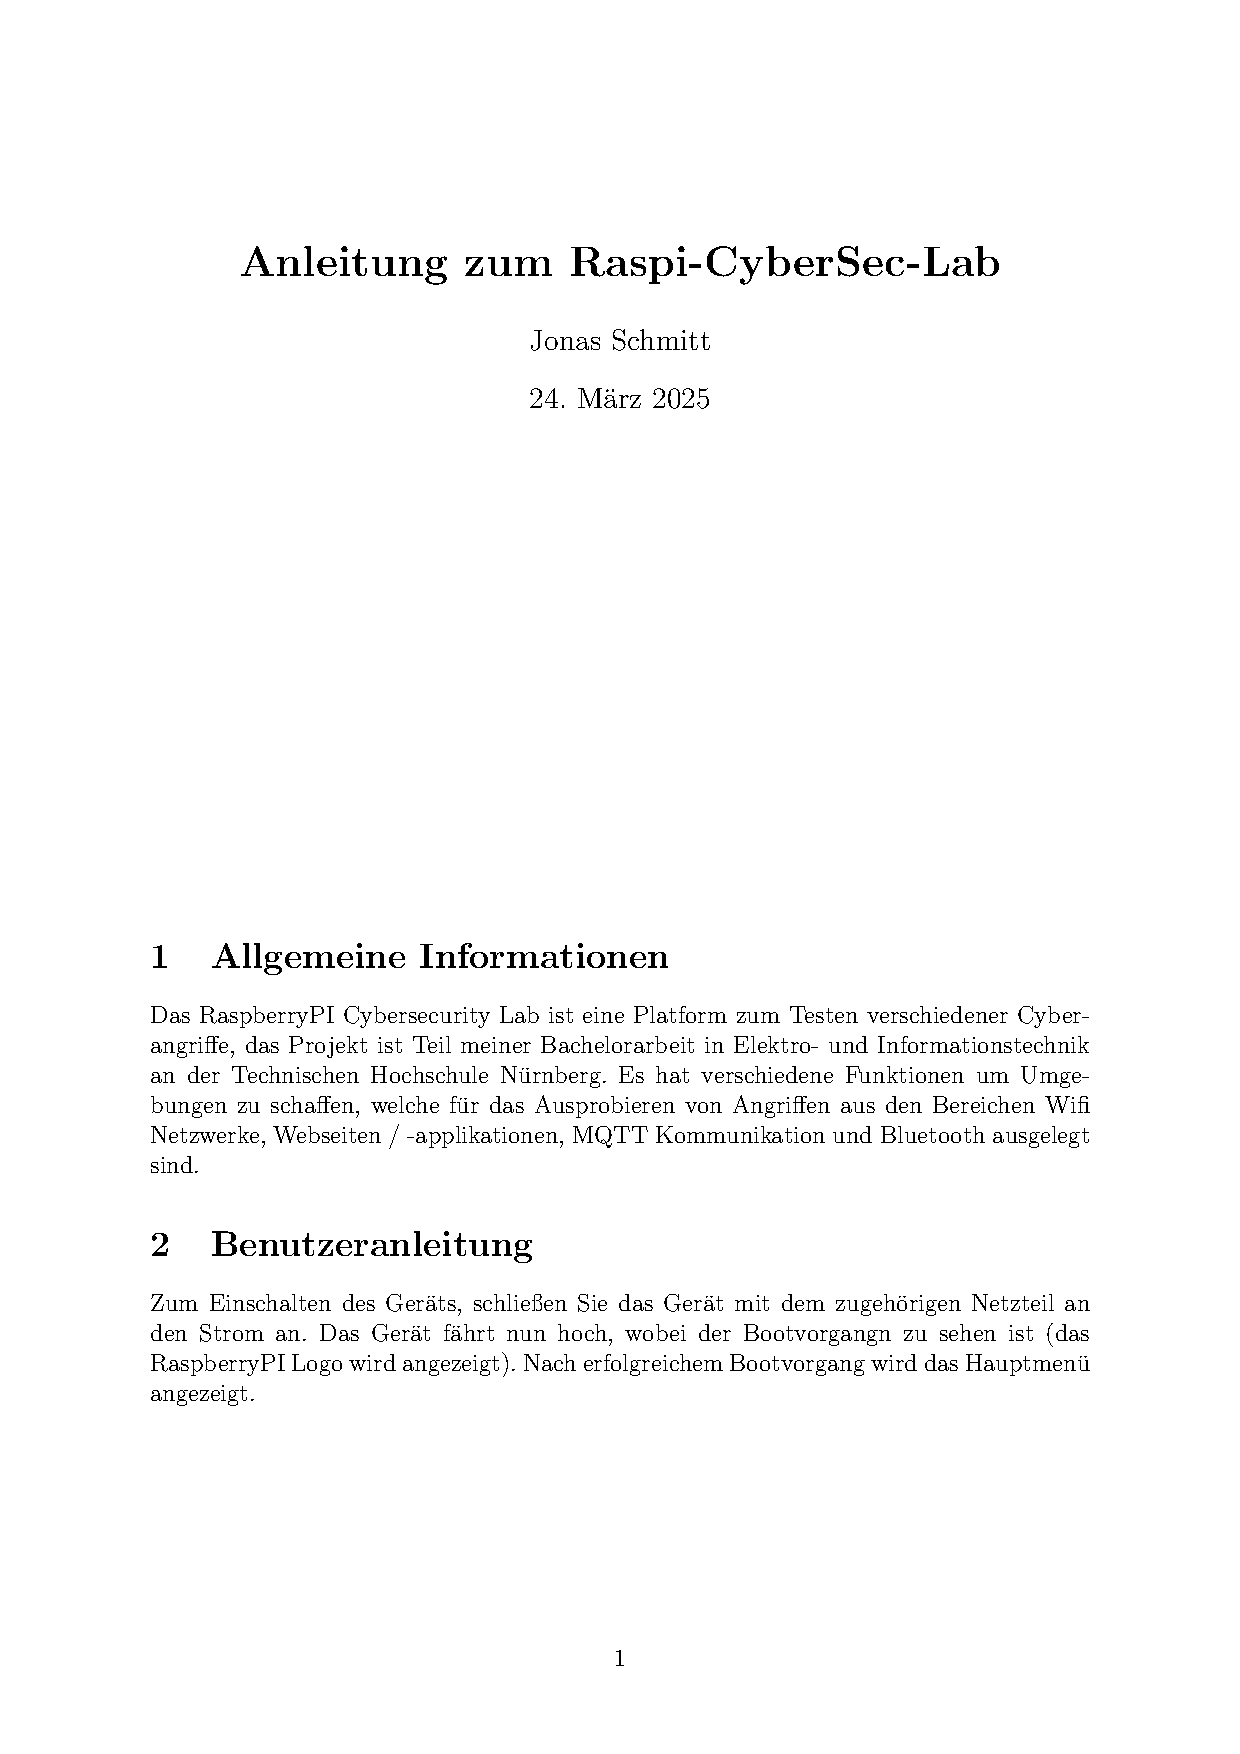
\includepdf[pages={1-}]{userguide/userguide.pdf}

\section{Documentation}
\begin{table}[h]
    \caption{menu and option overview}
    \label{tab:menues_options}
    \centering
    \ra{1.3}
    \small
        \begin{tabular}{@{}lrclclrclcl@{}}\toprule
            \multicolumn{11}{c}{Main Menu} \\
            \midrule
            \multicolumn{2}{c}{wifi} && \multicolumn{1}{c}{bluetooth} && \multicolumn{2}{c}{webapp} && development && power off \\
            \cmidrule{1-2} \cmidrule{4-4} \cmidrule{6-7} \cmidrule{9-9} 
            activate & WEP && \textit{under} && Juice Shop & on && option 1 && \\
            & WPA && \textit{development} &&& off && option 2\\
            & WPA2 &&&& MQTT & on && option 3\\
            & WPA3 &&&&& off && option 4\\
            deactivate &&&&&&&& option 5\\
            status\\
            new password & WEP\\
            & WPA\\
            & WPA2\\
            & WPA3\\
            monitor & on\\
            & off\\
            & show log\\
            & delete log\\
            \bottomrule
        \end{tabular}
\end{table}


\begin{figure}[h]
    
\includegraphics[width=0.25\linewidth]{figures/Abbildungen/hackerypi/menu_wifi.png}
    
\includegraphics[width=0.3\linewidth]{figures/Abbildungen/hackerypi/menu_webapp.png}
    
\includegraphics[width=0.35\linewidth]{figures/Abbildungen/hackerypi/menu_dev.png}
    \centering
    \caption{Device Menues}
    \label{fig:menues}
\end{figure}

\backmatter
\listoffigures
\cleardoublepage

\listoftables
\cleardoublepage

\renewcommand{\lstlistlistingname}{List of Listings}  % change for German thesis
\lstlistoflistings
\cleardoublepage

\bibliographystyle{wmaainf}
\bibliography{refs}

\printnoidxglossaries

\end{document}
